\documentclass[1p]{elsarticle_modified}
%\bibliographystyle{elsarticle-num}

%\usepackage[colorlinks]{hyperref}
%\usepackage{abbrmath_seonhwa} %\Abb, \Ascr, \Acal ,\Abf, \Afrak
\usepackage{amsfonts}
\usepackage{amssymb}
\usepackage{amsmath}
\usepackage{amsthm}
\usepackage{scalefnt}
\usepackage{amsbsy}
\usepackage{kotex}
\usepackage{caption}
\usepackage{subfig}
\usepackage{color}
\usepackage{graphicx}
\usepackage{xcolor} %% white, black, red, green, blue, cyan, magenta, yellow
\usepackage{float}
\usepackage{setspace}
\usepackage{hyperref}

\usepackage{tikz}
\usetikzlibrary{arrows}

\usepackage{multirow}
\usepackage{array} % fixed length table
\usepackage{hhline}

%%%%%%%%%%%%%%%%%%%%%
\makeatletter
\renewcommand*\env@matrix[1][\arraystretch]{%
	\edef\arraystretch{#1}%
	\hskip -\arraycolsep
	\let\@ifnextchar\new@ifnextchar
	\array{*\c@MaxMatrixCols c}}
\makeatother %https://tex.stackexchange.com/questions/14071/how-can-i-increase-the-line-spacing-in-a-matrix
%%%%%%%%%%%%%%%

\usepackage[normalem]{ulem}

\newcommand{\msout}[1]{\ifmmode\text{\sout{\ensuremath{#1}}}\else\sout{#1}\fi}
%SOURCE: \msout is \stkout macro in https://tex.stackexchange.com/questions/20609/strikeout-in-math-mode

\newcommand{\cancel}[1]{
	\ifmmode
	{\color{red}\msout{#1}}
	\else
	{\color{red}\sout{#1}}
	\fi
}

\newcommand{\add}[1]{
	{\color{blue}\uwave{#1}}
}

\newcommand{\replace}[2]{
	\ifmmode
	{\color{red}\msout{#1}}{\color{blue}\uwave{#2}}
	\else
	{\color{red}\sout{#1}}{\color{blue}\uwave{#2}}
	\fi
}

\newcommand{\Sol}{\mathcal{S}} %segment
\newcommand{\D}{D} %diagram
\newcommand{\A}{\mathcal{A}} %arc


%%%%%%%%%%%%%%%%%%%%%%%%%%%%%5 test

\def\sl{\operatorname{\textup{SL}}(2,\Cbb)}
\def\psl{\operatorname{\textup{PSL}}(2,\Cbb)}
\def\quan{\mkern 1mu \triangleright \mkern 1mu}

\theoremstyle{definition}
\newtheorem{thm}{Theorem}[section]
\newtheorem{prop}[thm]{Proposition}
\newtheorem{lem}[thm]{Lemma}
\newtheorem{ques}[thm]{Question}
\newtheorem{cor}[thm]{Corollary}
\newtheorem{defn}[thm]{Definition}
\newtheorem{exam}[thm]{Example}
\newtheorem{rmk}[thm]{Remark}
\newtheorem{alg}[thm]{Algorithm}

\newcommand{\I}{\sqrt{-1}}
\begin{document}

%\begin{frontmatter}
%
%\title{Boundary parabolic representations of knots up to 8 crossings}
%
%%% Group authors per affiliation:
%\author{Yunhi Cho} 
%\address{Department of Mathematics, University of Seoul, Seoul, Korea}
%\ead{yhcho@uos.ac.kr}
%
%
%\author{Seonhwa Kim} %\fnref{s_kim}}
%\address{Center for Geometry and Physics, Institute for Basic Science, Pohang, 37673, Korea}
%\ead{ryeona17@ibs.re.kr}
%
%\author{Hyuk Kim}
%\address{Department of Mathematical Sciences, Seoul National University, Seoul 08826, Korea}
%\ead{hyukkim@snu.ac.kr}
%
%\author{Seokbeom Yoon}
%\address{Department of Mathematical Sciences, Seoul National University, Seoul, 08826,  Korea}
%\ead{sbyoon15@snu.ac.kr}
%
%\begin{abstract}
%We find all boundary parabolic representation of knots up to 8 crossings.
%
%\end{abstract}
%\begin{keyword}
%    \MSC[2010] 57M25 
%\end{keyword}
%
%\end{frontmatter}

%\linenumbers
%\tableofcontents
%
\newcommand\colored[1]{\textcolor{white}{\rule[-0.35ex]{0.8em}{1.4ex}}\kern-0.8em\color{red} #1}%
%\newcommand\colored[1]{\textcolor{white}{ #1}\kern-2.17ex	\textcolor{white}{ #1}\kern-1.81ex	\textcolor{white}{ #1}\kern-2.15ex\color{red}#1	}

{\Large $\underline{12n_{0203}~(K12n_{0203})}$}

\setlength{\tabcolsep}{10pt}
\renewcommand{\arraystretch}{1.6}
\vspace{1cm}\begin{tabular}{m{100pt}>{\centering\arraybackslash}m{274pt}}
\multirow{5}{120pt}{
	\centering
	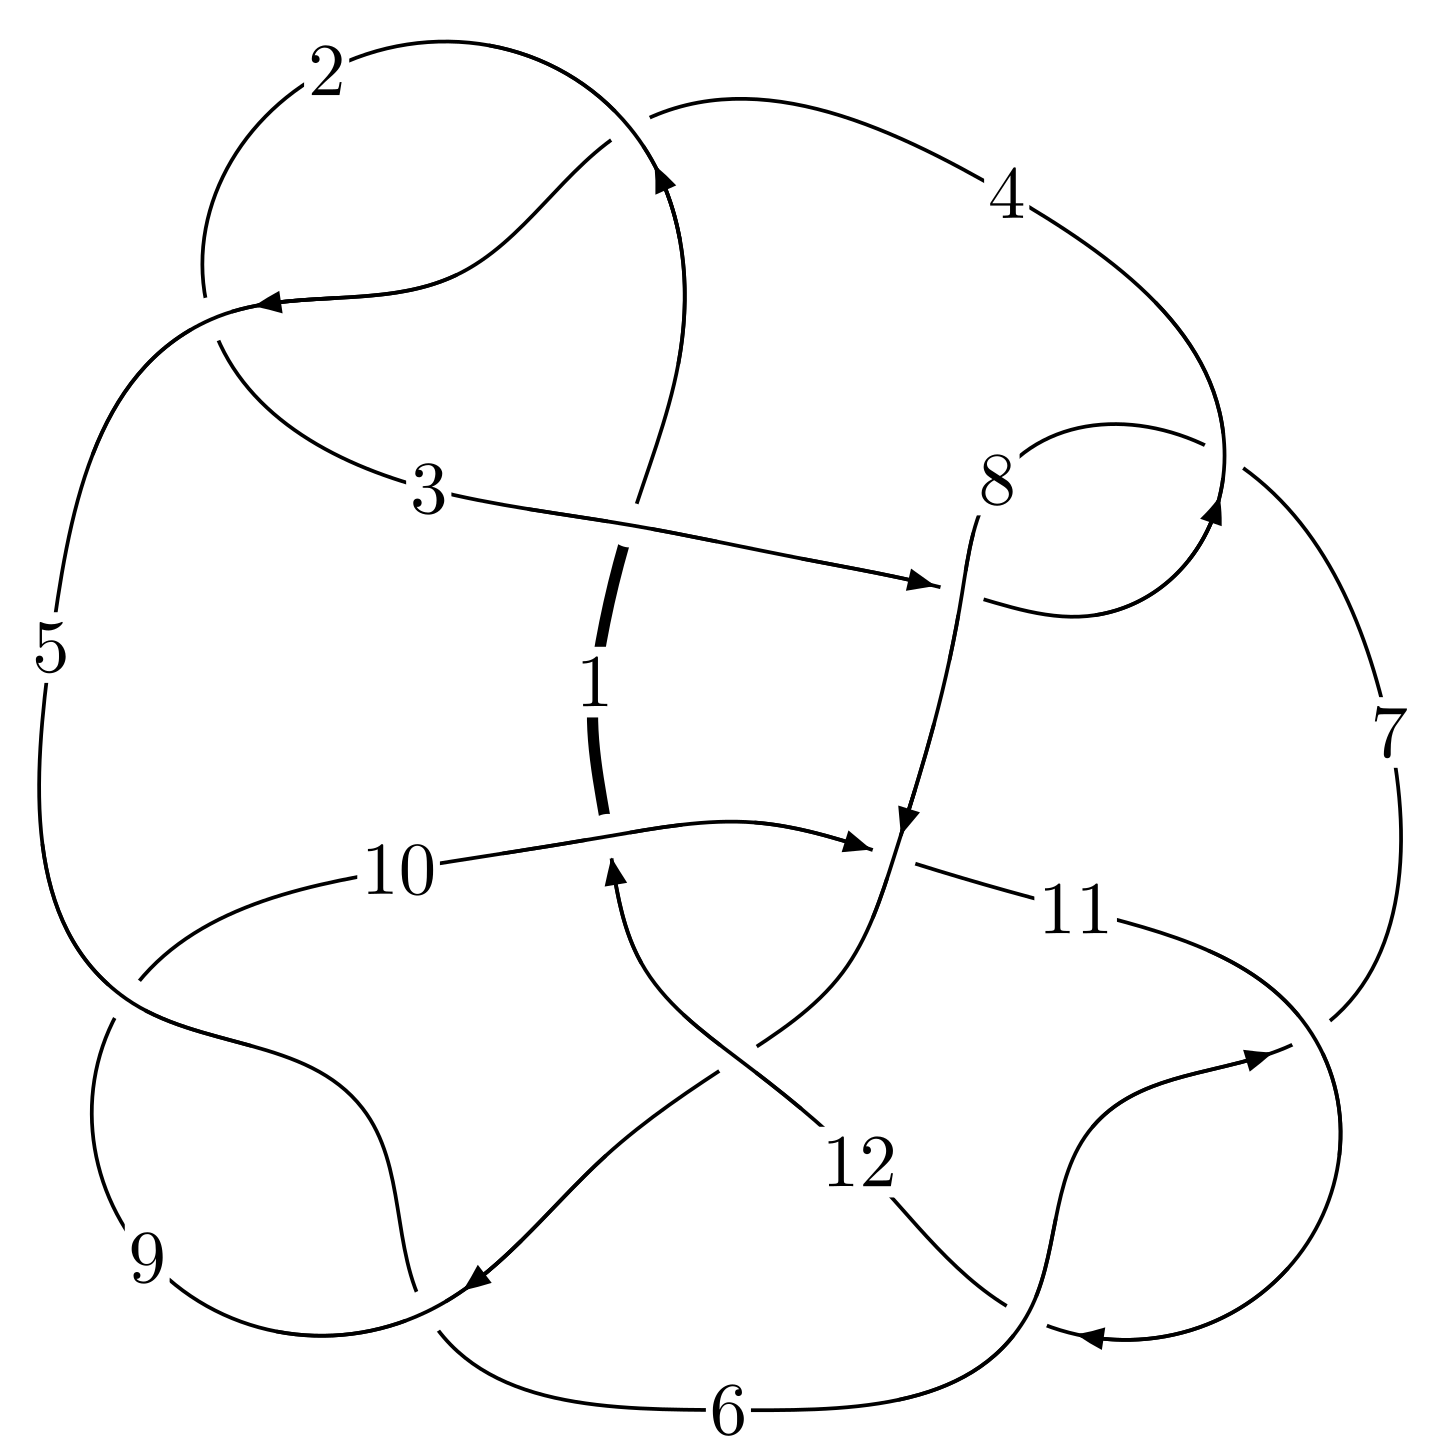
\includegraphics[width=112pt]{../../../GIT/diagram.site/Diagrams/png/2292_12n_0203.png}\\
\ \ \ A knot diagram\footnotemark}&
\allowdisplaybreaks
\textbf{Linearized knot diagam} \\
\cline{2-2}
 &
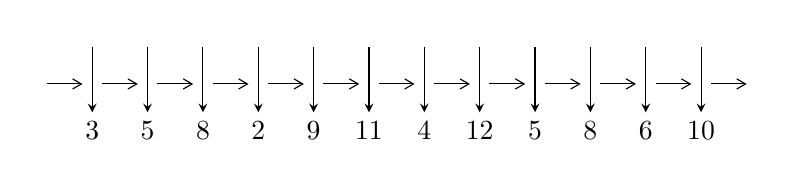
\begin{tikzpicture}[x=20pt, y=17pt]
	% nodes
	\node (C0) at (0, 0) {};
	\node (C1) at (1, 0) {};
	\node (C1U) at (1, +1) {};
	\node (C1D) at (1, -1) {3};

	\node (C2) at (2, 0) {};
	\node (C2U) at (2, +1) {};
	\node (C2D) at (2, -1) {5};

	\node (C3) at (3, 0) {};
	\node (C3U) at (3, +1) {};
	\node (C3D) at (3, -1) {8};

	\node (C4) at (4, 0) {};
	\node (C4U) at (4, +1) {};
	\node (C4D) at (4, -1) {2};

	\node (C5) at (5, 0) {};
	\node (C5U) at (5, +1) {};
	\node (C5D) at (5, -1) {9};

	\node (C6) at (6, 0) {};
	\node (C6U) at (6, +1) {};
	\node (C6D) at (6, -1) {11};

	\node (C7) at (7, 0) {};
	\node (C7U) at (7, +1) {};
	\node (C7D) at (7, -1) {4};

	\node (C8) at (8, 0) {};
	\node (C8U) at (8, +1) {};
	\node (C8D) at (8, -1) {12};

	\node (C9) at (9, 0) {};
	\node (C9U) at (9, +1) {};
	\node (C9D) at (9, -1) {5};

	\node (C10) at (10, 0) {};
	\node (C10U) at (10, +1) {};
	\node (C10D) at (10, -1) {8};

	\node (C11) at (11, 0) {};
	\node (C11U) at (11, +1) {};
	\node (C11D) at (11, -1) {6};

	\node (C12) at (12, 0) {};
	\node (C12U) at (12, +1) {};
	\node (C12D) at (12, -1) {10};
	\node (C13) at (13, 0) {};

	% arrows
	\draw[->,>={angle 60}]
	(C0) edge (C1) (C1) edge (C2) (C2) edge (C3) (C3) edge (C4) (C4) edge (C5) (C5) edge (C6) (C6) edge (C7) (C7) edge (C8) (C8) edge (C9) (C9) edge (C10) (C10) edge (C11) (C11) edge (C12) (C12) edge (C13) ;	\draw[->,>=stealth]
	(C1U) edge (C1D) (C2U) edge (C2D) (C3U) edge (C3D) (C4U) edge (C4D) (C5U) edge (C5D) (C6U) edge (C6D) (C7U) edge (C7D) (C8U) edge (C8D) (C9U) edge (C9D) (C10U) edge (C10D) (C11U) edge (C11D) (C12U) edge (C12D) ;
	\end{tikzpicture} \\
\hhline{~~} \\& 
\textbf{Solving Sequence} \\ \cline{2-2} 
 &
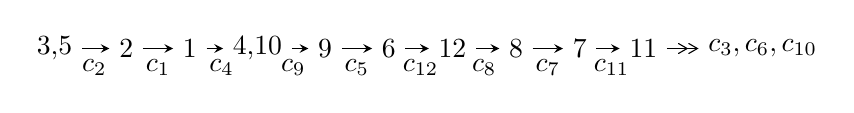
\begin{tikzpicture}[x=23pt, y=7pt]
	% node
	\node (A0) at (-1/8, 0) {3,5};
	\node (A1) at (1, 0) {2};
	\node (A2) at (2, 0) {1};
	\node (A3) at (49/16, 0) {4,10};
	\node (A4) at (33/8, 0) {9};
	\node (A5) at (41/8, 0) {6};
	\node (A6) at (49/8, 0) {12};
	\node (A7) at (57/8, 0) {8};
	\node (A8) at (65/8, 0) {7};
	\node (A9) at (73/8, 0) {11};
	\node (C1) at (1/2, -1) {$c_{2}$};
	\node (C2) at (3/2, -1) {$c_{1}$};
	\node (C3) at (5/2, -1) {$c_{4}$};
	\node (C4) at (29/8, -1) {$c_{9}$};
	\node (C5) at (37/8, -1) {$c_{5}$};
	\node (C6) at (45/8, -1) {$c_{12}$};
	\node (C7) at (53/8, -1) {$c_{8}$};
	\node (C8) at (61/8, -1) {$c_{7}$};
	\node (C9) at (69/8, -1) {$c_{11}$};
	\node (A10) at (11, 0) {$c_{3},c_{6},c_{10}$};

	% edge
	\draw[->,>=stealth]	
	(A0) edge (A1) (A1) edge (A2) (A2) edge (A3) (A3) edge (A4) (A4) edge (A5) (A5) edge (A6) (A6) edge (A7) (A7) edge (A8) (A8) edge (A9) ;
	\draw[->>,>={angle 60}]	
	(A9) edge (A10);
\end{tikzpicture} \\ 

\end{tabular} \\

\footnotetext{
The image of knot diagram is generated by the software ``\textbf{Draw programme}" developed by Andrew Bartholomew(\url{http://www.layer8.co.uk/maths/draw/index.htm\#Running-draw}), where we modified some parts for our purpose(\url{https://github.com/CATsTAILs/LinksPainter}).
}\phantom \\ \newline 
\centering \textbf{Ideals for irreducible components\footnotemark of $X_{\text{par}}$} 
 
\begin{align*}
I^u_{1}&=\langle 
-51478029223711 u^{17}-94965699826026 u^{16}+\cdots+9603901893745904 b-98088892223296,\\
\phantom{I^u_{1}}&\phantom{= \langle  }-2.34490\times10^{14} u^{17}-5.69398\times10^{14} u^{16}+\cdots+9.60390\times10^{15} a-3.43754\times10^{16},\\
\phantom{I^u_{1}}&\phantom{= \langle  }u^{18}+5 u^{17}+\cdots-108 u+16\rangle \\
I^u_{2}&=\langle 
- u^{11}-4 u^{10}-3 u^9+5 u^8+7 u^7-2 u^6-4 u^5+u^4+2 u^3+u^2+b+u,\\
\phantom{I^u_{2}}&\phantom{= \langle  }- u^{11}-4 u^{10}-2 u^9+9 u^8+11 u^7-3 u^6-8 u^5-2 u^4-2 u^3- u^2+a+2 u+1,\\
\phantom{I^u_{2}}&\phantom{= \langle  }u^{12}+5 u^{11}+7 u^{10}-3 u^9-17 u^8-13 u^7+4 u^6+12 u^5+8 u^4+2 u^3-2 u^2-2 u-1\rangle \\
I^u_{3}&=\langle 
a^2+2 b- a+2,\;a^3+2 a+1,\;u-1\rangle \\
I^u_{4}&=\langle 
-14 a^3 u+5 a^3-10 a^2 u+8 a^2+27 a u+31 b-3 a+12 u+9,\\
\phantom{I^u_{4}}&\phantom{= \langle  }a^4+a^3+6 a^2 u+14 a^2+6 a u+14 a+30 u+73,\;u^2+2 u-1\rangle \\
I^u_{5}&=\langle 
- a^3+b-2 a+1,\;a^4- a^3+2 a^2-2 a+1,\;u-1\rangle \\
\\
\end{align*}
\raggedright * 5 irreducible components of $\dim_{\mathbb{C}}=0$, with total 45 representations.\\
\footnotetext{All coefficients of polynomials are rational numbers. But the coefficients are sometimes approximated in decimal forms when there is not enough margin.}
\newpage
\renewcommand{\arraystretch}{1}
\centering \section*{I. $I^u_{1}= \langle -5.15\times10^{13} u^{17}-9.50\times10^{13} u^{16}+\cdots+9.60\times10^{15} b-9.81\times10^{13},\;-2.34\times10^{14} u^{17}-5.69\times10^{14} u^{16}+\cdots+9.60\times10^{15} a-3.44\times10^{16},\;u^{18}+5 u^{17}+\cdots-108 u+16 \rangle$}
\flushleft \textbf{(i) Arc colorings}\\
\begin{tabular}{m{7pt} m{180pt} m{7pt} m{180pt} }
\flushright $a_{3}=$&$\begin{pmatrix}1\\0\end{pmatrix}$ \\
\flushright $a_{5}=$&$\begin{pmatrix}0\\u\end{pmatrix}$ \\
\flushright $a_{2}=$&$\begin{pmatrix}1\\- u^2\end{pmatrix}$ \\
\flushright $a_{1}=$&$\begin{pmatrix}- u^2+1\\- u^2\end{pmatrix}$ \\
\flushright $a_{4}=$&$\begin{pmatrix}u\\- u^3+u\end{pmatrix}$ \\
\flushright $a_{10}=$&$\begin{pmatrix}0.0244161 u^{17}+0.0592882 u^{16}+\cdots-2.08611 u+3.57931\\0.00536012 u^{17}+0.00988824 u^{16}+\cdots-2.52686 u+0.0102134\end{pmatrix}$ \\
\flushright $a_{9}=$&$\begin{pmatrix}0.0244161 u^{17}+0.0592882 u^{16}+\cdots-2.08611 u+3.57931\\-0.0722239 u^{17}-0.275667 u^{16}+\cdots+4.64539 u-0.994467\end{pmatrix}$ \\
\flushright $a_{6}=$&$\begin{pmatrix}-0.00210596 u^{17}-0.0126160 u^{16}+\cdots+1.37231 u-1.55076\\-0.0194628 u^{17}-0.0641489 u^{16}+\cdots+1.60320 u+0.0763384\end{pmatrix}$ \\
\flushright $a_{12}=$&$\begin{pmatrix}0.00368464 u^{17}+0.0157751 u^{16}+\cdots-1.75467 u+2.18995\\-0.0138662 u^{17}-0.0634618 u^{16}+\cdots-0.358806 u-0.0322530\end{pmatrix}$ \\
\flushright $a_{8}=$&$\begin{pmatrix}-0.0979771 u^{17}-0.396405 u^{16}+\cdots+9.53653 u+1.24502\\0.0102874 u^{17}+0.0611624 u^{16}+\cdots-2.32701 u-0.0719485\end{pmatrix}$ \\
\flushright $a_{7}=$&$\begin{pmatrix}-0.0882516 u^{17}-0.373557 u^{16}+\cdots+10.5756 u+1.08043\\-0.0373820 u^{17}-0.114869 u^{16}+\cdots+1.65191 u-0.649024\end{pmatrix}$ \\
\flushright $a_{11}=$&$\begin{pmatrix}-0.126113 u^{17}-0.483663 u^{16}+\cdots+11.1577 u+1.06434\\0.0672052 u^{17}+0.236972 u^{16}+\cdots-8.81033 u+0.956875\end{pmatrix}$\\&\end{tabular}
\flushleft \textbf{(ii) Obstruction class $= -1$}\\~\\
\flushleft \textbf{(iii) Cusp Shapes $= -\frac{7248898902357663}{38415607574983616} u^{17}-\frac{19550123270823501}{19207803787491808} u^{16}+\cdots-\frac{53749314921709817}{9603901893745904} u-\frac{32406067335746281}{2400975473436476}$}\\~\\
\newpage\renewcommand{\arraystretch}{1}
\flushleft \textbf{(iv) u-Polynomials at the component}\newline \\
\begin{tabular}{m{50pt}|m{274pt}}
Crossings & \hspace{64pt}u-Polynomials at each crossing \\
\hline $$\begin{aligned}c_{1}\end{aligned}$$&$\begin{aligned}
&u^{18}+19 u^{17}+\cdots+15984 u+256
\end{aligned}$\\
\hline $$\begin{aligned}c_{2},c_{4}\end{aligned}$$&$\begin{aligned}
&u^{18}-5 u^{17}+\cdots+108 u+16
\end{aligned}$\\
\hline $$\begin{aligned}c_{3},c_{7}\end{aligned}$$&$\begin{aligned}
&u^{18}-9 u^{16}+\cdots-160 u-128
\end{aligned}$\\
\hline $$\begin{aligned}c_{5},c_{6},c_{9}\\c_{11}\end{aligned}$$&$\begin{aligned}
&u^{18}+4 u^{16}+\cdots+u-1
\end{aligned}$\\
\hline $$\begin{aligned}c_{8}\end{aligned}$$&$\begin{aligned}
&u^{18}+9 u^{17}+\cdots+28 u+4
\end{aligned}$\\
\hline $$\begin{aligned}c_{10},c_{12}\end{aligned}$$&$\begin{aligned}
&u^{18}-4 u^{17}+\cdots-13 u+1
\end{aligned}$\\
\hline
\end{tabular}\\~\\
\newpage\renewcommand{\arraystretch}{1}
\flushleft \textbf{(v) Riley Polynomials at the component}\newline \\
\begin{tabular}{m{50pt}|m{274pt}}
Crossings & \hspace{64pt}Riley Polynomials at each crossing \\
\hline $$\begin{aligned}c_{1}\end{aligned}$$&$\begin{aligned}
&y^{18}+13 y^{17}+\cdots-211267328 y+65536
\end{aligned}$\\
\hline $$\begin{aligned}c_{2},c_{4}\end{aligned}$$&$\begin{aligned}
&y^{18}-19 y^{17}+\cdots-15984 y+256
\end{aligned}$\\
\hline $$\begin{aligned}c_{3},c_{7}\end{aligned}$$&$\begin{aligned}
&y^{18}-18 y^{17}+\cdots-257024 y+16384
\end{aligned}$\\
\hline $$\begin{aligned}c_{5},c_{6},c_{9}\\c_{11}\end{aligned}$$&$\begin{aligned}
&y^{18}+8 y^{17}+\cdots-13 y+1
\end{aligned}$\\
\hline $$\begin{aligned}c_{8}\end{aligned}$$&$\begin{aligned}
&y^{18}+3 y^{17}+\cdots+88 y+16
\end{aligned}$\\
\hline $$\begin{aligned}c_{10},c_{12}\end{aligned}$$&$\begin{aligned}
&y^{18}-12 y^{17}+\cdots-27 y+1
\end{aligned}$\\
\hline
\end{tabular}\\~\\
\newpage\flushleft \textbf{(vi) Complex Volumes and Cusp Shapes}
$$\begin{array}{c|c|c}  
\text{Solutions to }I^u_{1}& \I (\text{vol} + \sqrt{-1}CS) & \text{Cusp shape}\\
 \hline 
\begin{aligned}
u &= -0.498072 + 0.803560 I \\
a &= \phantom{-}0.804411 - 0.072881 I \\
b &= \phantom{-}0.601639 + 0.155591 I\end{aligned}
 & \phantom{-}3.85179 + 0.21064 I & -8.48737 - 0.11416 I \\ \hline\begin{aligned}
u &= -0.498072 - 0.803560 I \\
a &= \phantom{-}0.804411 + 0.072881 I \\
b &= \phantom{-}0.601639 - 0.155591 I\end{aligned}
 & \phantom{-}3.85179 - 0.21064 I & -8.48737 + 0.11416 I \\ \hline\begin{aligned}
u &= \phantom{-}0.854940\phantom{ +0.000000I} \\
a &= -0.328563\phantom{ +0.000000I} \\
b &= -2.47470\phantom{ +0.000000I}\end{aligned}
 & -2.86169\phantom{ +0.000000I} & -58.1310\phantom{ +0.000000I} \\ \hline\begin{aligned}
u &= \phantom{-}0.731104 + 0.323621 I \\
a &= \phantom{-}0.210674 - 0.558567 I \\
b &= -0.567133 + 0.114177 I\end{aligned}
 & -0.825090 - 0.258812 I & -11.03204 - 0.79258 I \\ \hline\begin{aligned}
u &= \phantom{-}0.731104 - 0.323621 I \\
a &= \phantom{-}0.210674 + 0.558567 I \\
b &= -0.567133 - 0.114177 I\end{aligned}
 & -0.825090 + 0.258812 I & -11.03204 + 0.79258 I \\ \hline\begin{aligned}
u &= -1.067010 + 0.610706 I \\
a &= -0.142436 + 0.567488 I \\
b &= -0.526588 + 0.193604 I\end{aligned}
 & \phantom{-}2.12814 + 5.07138 I & -8.91832 - 8.83616 I \\ \hline\begin{aligned}
u &= -1.067010 - 0.610706 I \\
a &= -0.142436 - 0.567488 I \\
b &= -0.526588 - 0.193604 I\end{aligned}
 & \phantom{-}2.12814 - 5.07138 I & -8.91832 + 8.83616 I \\ \hline\begin{aligned}
u &= -1.236400 + 0.168858 I \\
a &= \phantom{-}0.057682 + 1.280350 I \\
b &= \phantom{-}0.079988 + 0.291227 I\end{aligned}
 & \phantom{-}7.38910 - 4.84420 I & -12.25477 - 0.83439 I \\ \hline\begin{aligned}
u &= -1.236400 - 0.168858 I \\
a &= \phantom{-}0.057682 - 1.280350 I \\
b &= \phantom{-}0.079988 - 0.291227 I\end{aligned}
 & \phantom{-}7.38910 + 4.84420 I & -12.25477 + 0.83439 I \\ \hline\begin{aligned}
u &= \phantom{-}1.41842 + 0.74975 I \\
a &= -0.720025 + 0.318355 I \\
b &= -1.45615 + 0.15501 I\end{aligned}
 & -3.70938 + 0.73390 I & -13.05363 - 1.20335 I\\
 \hline 
 \end{array}$$\newpage$$\begin{array}{c|c|c}  
\text{Solutions to }I^u_{1}& \I (\text{vol} + \sqrt{-1}CS) & \text{Cusp shape}\\
 \hline 
\begin{aligned}
u &= \phantom{-}1.41842 - 0.74975 I \\
a &= -0.720025 - 0.318355 I \\
b &= -1.45615 - 0.15501 I\end{aligned}
 & -3.70938 - 0.73390 I & -13.05363 + 1.20335 I \\ \hline\begin{aligned}
u &= \phantom{-}1.22478 + 1.30063 I \\
a &= \phantom{-}0.896477 - 0.274017 I \\
b &= \phantom{-}1.44915 - 0.14091 I\end{aligned}
 & -2.93065 - 5.27680 I & -11.38955 + 3.92982 I \\ \hline\begin{aligned}
u &= \phantom{-}1.22478 - 1.30063 I \\
a &= \phantom{-}0.896477 + 0.274017 I \\
b &= \phantom{-}1.44915 + 0.14091 I\end{aligned}
 & -2.93065 + 5.27680 I & -11.38955 - 3.92982 I \\ \hline\begin{aligned}
u &= -1.73766 + 0.57784 I \\
a &= \phantom{-}0.621844 - 0.638194 I \\
b &= \phantom{-}1.94004 - 0.09952 I\end{aligned}
 & -12.9639 + 5.8348 I & -10.78539 - 2.21152 I \\ \hline\begin{aligned}
u &= -1.73766 - 0.57784 I \\
a &= \phantom{-}0.621844 + 0.638194 I \\
b &= \phantom{-}1.94004 + 0.09952 I\end{aligned}
 & -12.9639 - 5.8348 I & -10.78539 + 2.21152 I \\ \hline\begin{aligned}
u &= \phantom{-}0.132712\phantom{ +0.000000I} \\
a &= \phantom{-}3.15830\phantom{ +0.000000I} \\
b &= -0.353393\phantom{ +0.000000I}\end{aligned}
 & -0.661114\phantom{ +0.000000I} & -14.7530\phantom{ +0.000000I} \\ \hline\begin{aligned}
u &= -1.82899 + 0.67910 I \\
a &= -0.768496 + 0.689009 I \\
b &= -2.10690 + 0.22733 I\end{aligned}
 & -11.7403 + 13.7046 I & -10.51182 - 5.40024 I \\ \hline\begin{aligned}
u &= -1.82899 - 0.67910 I \\
a &= -0.768496 - 0.689009 I \\
b &= -2.10690 - 0.22733 I\end{aligned}
 & -11.7403 - 13.7046 I & -10.51182 + 5.40024 I\\
 \hline 
 \end{array}$$\newpage\newpage\renewcommand{\arraystretch}{1}
\centering \section*{II. $I^u_{2}= \langle - u^{11}-4 u^{10}+\cdots+b+u,\;- u^{11}-4 u^{10}+\cdots+a+1,\;u^{12}+5 u^{11}+\cdots-2 u-1 \rangle$}
\flushleft \textbf{(i) Arc colorings}\\
\begin{tabular}{m{7pt} m{180pt} m{7pt} m{180pt} }
\flushright $a_{3}=$&$\begin{pmatrix}1\\0\end{pmatrix}$ \\
\flushright $a_{5}=$&$\begin{pmatrix}0\\u\end{pmatrix}$ \\
\flushright $a_{2}=$&$\begin{pmatrix}1\\- u^2\end{pmatrix}$ \\
\flushright $a_{1}=$&$\begin{pmatrix}- u^2+1\\- u^2\end{pmatrix}$ \\
\flushright $a_{4}=$&$\begin{pmatrix}u\\- u^3+u\end{pmatrix}$ \\
\flushright $a_{10}=$&$\begin{pmatrix}u^{11}+4 u^{10}+2 u^9-9 u^8-11 u^7+3 u^6+8 u^5+2 u^4+2 u^3+u^2-2 u-1\\u^{11}+4 u^{10}+3 u^9-5 u^8-7 u^7+2 u^6+4 u^5- u^4-2 u^3- u^2- u\end{pmatrix}$ \\
\flushright $a_{9}=$&$\begin{pmatrix}u^{11}+4 u^{10}+2 u^9-9 u^8-11 u^7+3 u^6+8 u^5+2 u^4+2 u^3+u^2-2 u-1\\u^{11}+3 u^{10}-4 u^8+2 u^7+8 u^6-2 u^5-8 u^4-4 u^3+1\end{pmatrix}$ \\
\flushright $a_{6}=$&$\begin{pmatrix}u^{11}+5 u^{10}+\cdots-4 u-3\\u^{10}+4 u^9+2 u^8-9 u^7-12 u^6+7 u^4+4 u^3+2 u^2- u-1\end{pmatrix}$ \\
\flushright $a_{12}=$&$\begin{pmatrix}- u^{11}-5 u^{10}+\cdots+3 u+3\\- u^{11}-5 u^{10}-8 u^9-2 u^8+9 u^7+11 u^6+5 u^5- u^4-4 u^3-5 u^2- u\end{pmatrix}$ \\
\flushright $a_{8}=$&$\begin{pmatrix}-2 u^{11}-8 u^{10}-6 u^9+12 u^8+22 u^7+3 u^6-14 u^5-10 u^4- u^3+2 u+1\\u^8+3 u^7-5 u^5-3 u^4+2 u^3+u^2+u\end{pmatrix}$ \\
\flushright $a_{7}=$&$\begin{pmatrix}-2 u^{11}-8 u^{10}-5 u^9+15 u^8+22 u^7-2 u^6-17 u^5-8 u^4+u^2+2 u+1\\- u^{11}-3 u^{10}+u^9+9 u^8+6 u^7-7 u^6-9 u^5-2 u^4+3 u^3+2 u^2+u\end{pmatrix}$ \\
\flushright $a_{11}=$&$\begin{pmatrix}u^{11}+4 u^{10}+2 u^9-9 u^8-11 u^7+3 u^6+8 u^5+2 u^4+2 u^3-2 u\\u^{11}+4 u^{10}+3 u^9-5 u^8-7 u^7+2 u^6+4 u^5- u^3-2 u^2-2 u\end{pmatrix}$\\&\end{tabular}
\flushleft \textbf{(ii) Obstruction class $= 1$}\\~\\
\flushleft \textbf{(iii) Cusp Shapes $= u^{11}+3 u^{10}+2 u^9-7 u^7-16 u^6-15 u^5+5 u^4+10 u^3+10 u^2+5 u-2$}\\~\\
\newpage\renewcommand{\arraystretch}{1}
\flushleft \textbf{(iv) u-Polynomials at the component}\newline \\
\begin{tabular}{m{50pt}|m{274pt}}
Crossings & \hspace{64pt}u-Polynomials at each crossing \\
\hline $$\begin{aligned}c_{1}\end{aligned}$$&$\begin{aligned}
&u^{12}-11 u^{11}+\cdots-4 u^2+1
\end{aligned}$\\
\hline $$\begin{aligned}c_{2}\end{aligned}$$&$\begin{aligned}
&u^{12}+5 u^{11}+\cdots-2 u-1
\end{aligned}$\\
\hline $$\begin{aligned}c_{3}\end{aligned}$$&$\begin{aligned}
&u^{12}+4 u^{11}+\cdots-2 u-1
\end{aligned}$\\
\hline $$\begin{aligned}c_{4}\end{aligned}$$&$\begin{aligned}
&u^{12}-5 u^{11}+\cdots+2 u-1
\end{aligned}$\\
\hline $$\begin{aligned}c_{5},c_{11}\end{aligned}$$&$\begin{aligned}
&u^{12}+4 u^{10}+\cdots-7 u+1
\end{aligned}$\\
\hline $$\begin{aligned}c_{6},c_{9}\end{aligned}$$&$\begin{aligned}
&u^{12}+4 u^{10}+\cdots+7 u+1
\end{aligned}$\\
\hline $$\begin{aligned}c_{7}\end{aligned}$$&$\begin{aligned}
&u^{12}-4 u^{11}+\cdots+2 u-1
\end{aligned}$\\
\hline $$\begin{aligned}c_{8}\end{aligned}$$&$\begin{aligned}
&u^{12}+3 u^{11}+5 u^{10}+2 u^9- u^8-4 u^7+3 u^6+3 u^4-6 u^3-2 u^2-4 u+1
\end{aligned}$\\
\hline $$\begin{aligned}c_{10},c_{12}\end{aligned}$$&$\begin{aligned}
&u^{12}+4 u^{11}-2 u^{10}+6 u^9+3 u^8+3 u^6+4 u^5- u^4-2 u^3+5 u^2-3 u+1
\end{aligned}$\\
\hline
\end{tabular}\\~\\
\newpage\renewcommand{\arraystretch}{1}
\flushleft \textbf{(v) Riley Polynomials at the component}\newline \\
\begin{tabular}{m{50pt}|m{274pt}}
Crossings & \hspace{64pt}Riley Polynomials at each crossing \\
\hline $$\begin{aligned}c_{1}\end{aligned}$$&$\begin{aligned}
&y^{12}-31 y^{11}+\cdots-8 y+1
\end{aligned}$\\
\hline $$\begin{aligned}c_{2},c_{4}\end{aligned}$$&$\begin{aligned}
&y^{12}-11 y^{11}+\cdots-4 y^2+1
\end{aligned}$\\
\hline $$\begin{aligned}c_{3},c_{7}\end{aligned}$$&$\begin{aligned}
&y^{12}-6 y^{11}+\cdots+4 y+1
\end{aligned}$\\
\hline $$\begin{aligned}c_{5},c_{6},c_{9}\\c_{11}\end{aligned}$$&$\begin{aligned}
&y^{12}+8 y^{11}+\cdots-69 y+1
\end{aligned}$\\
\hline $$\begin{aligned}c_{8}\end{aligned}$$&$\begin{aligned}
&y^{12}+y^{11}+\cdots-20 y+1
\end{aligned}$\\
\hline $$\begin{aligned}c_{10},c_{12}\end{aligned}$$&$\begin{aligned}
&y^{12}-20 y^{11}+\cdots+y+1
\end{aligned}$\\
\hline
\end{tabular}\\~\\
\newpage\flushleft \textbf{(vi) Complex Volumes and Cusp Shapes}
$$\begin{array}{c|c|c}  
\text{Solutions to }I^u_{2}& \I (\text{vol} + \sqrt{-1}CS) & \text{Cusp shape}\\
 \hline 
\begin{aligned}
u &= \phantom{-}1.057460 + 0.095971 I \\
a &= -0.406859 - 1.196210 I \\
b &= -3.90485 + 1.89018 I\end{aligned}
 & \phantom{-}3.16210 - 2.20591 I & -7.78632 - 10.61857 I \\ \hline\begin{aligned}
u &= \phantom{-}1.057460 - 0.095971 I \\
a &= -0.406859 + 1.196210 I \\
b &= -3.90485 - 1.89018 I\end{aligned}
 & \phantom{-}3.16210 + 2.20591 I & -7.78632 + 10.61857 I \\ \hline\begin{aligned}
u &= -1.069100 + 0.511997 I \\
a &= -0.555353 + 0.877193 I \\
b &= -0.927124 - 0.102377 I\end{aligned}
 & \phantom{-}4.24653 + 6.29114 I & -8.72473 - 7.60786 I \\ \hline\begin{aligned}
u &= -1.069100 - 0.511997 I \\
a &= -0.555353 - 0.877193 I \\
b &= -0.927124 + 0.102377 I\end{aligned}
 & \phantom{-}4.24653 - 6.29114 I & -8.72473 + 7.60786 I \\ \hline\begin{aligned}
u &= \phantom{-}0.716863\phantom{ +0.000000I} \\
a &= -0.162026\phantom{ +0.000000I} \\
b &= -1.91362\phantom{ +0.000000I}\end{aligned}
 & -2.72064\phantom{ +0.000000I} & \phantom{-}6.26870\phantom{ +0.000000I} \\ \hline\begin{aligned}
u &= -0.462027 + 0.528026 I \\
a &= \phantom{-}1.05312 - 1.37955 I \\
b &= \phantom{-}0.804945 - 0.512875 I\end{aligned}
 & \phantom{-}6.06972 - 2.00606 I & -4.60411 + 0.72202 I \\ \hline\begin{aligned}
u &= -0.462027 - 0.528026 I \\
a &= \phantom{-}1.05312 + 1.37955 I \\
b &= \phantom{-}0.804945 + 0.512875 I\end{aligned}
 & \phantom{-}6.06972 + 2.00606 I & -4.60411 - 0.72202 I \\ \hline\begin{aligned}
u &= -1.154720 + 0.677187 I \\
a &= -0.051735 - 0.619586 I \\
b &= -0.108869 - 0.166947 I\end{aligned}
 & \phantom{-}2.03383 + 4.28434 I & -10.27189 + 0.84720 I \\ \hline\begin{aligned}
u &= -1.154720 - 0.677187 I \\
a &= -0.051735 + 0.619586 I \\
b &= -0.108869 + 0.166947 I\end{aligned}
 & \phantom{-}2.03383 - 4.28434 I & -10.27189 - 0.84720 I \\ \hline\begin{aligned}
u &= -0.034452 + 0.645190 I \\
a &= -1.85887 - 0.62285 I \\
b &= -0.388161 + 0.546694 I\end{aligned}
 & \phantom{-}5.19852 + 1.22317 I & -3.65798 - 0.64482 I\\
 \hline 
 \end{array}$$\newpage$$\begin{array}{c|c|c}  
\text{Solutions to }I^u_{2}& \I (\text{vol} + \sqrt{-1}CS) & \text{Cusp shape}\\
 \hline 
\begin{aligned}
u &= -0.034452 - 0.645190 I \\
a &= -1.85887 + 0.62285 I \\
b &= -0.388161 - 0.546694 I\end{aligned}
 & \phantom{-}5.19852 - 1.22317 I & -3.65798 + 0.64482 I \\ \hline\begin{aligned}
u &= -2.39117\phantom{ +0.000000I} \\
a &= \phantom{-}0.801439\phantom{ +0.000000I} \\
b &= \phantom{-}1.96174\phantom{ +0.000000I}\end{aligned}
 & -15.6717\phantom{ +0.000000I} & -10.1790\phantom{ +0.000000I}\\
 \hline 
 \end{array}$$\newpage\newpage\renewcommand{\arraystretch}{1}
\centering \section*{III. $I^u_{3}= \langle a^2+2 b- a+2,\;a^3+2 a+1,\;u-1 \rangle$}
\flushleft \textbf{(i) Arc colorings}\\
\begin{tabular}{m{7pt} m{180pt} m{7pt} m{180pt} }
\flushright $a_{3}=$&$\begin{pmatrix}1\\0\end{pmatrix}$ \\
\flushright $a_{5}=$&$\begin{pmatrix}0\\1\end{pmatrix}$ \\
\flushright $a_{2}=$&$\begin{pmatrix}1\\-1\end{pmatrix}$ \\
\flushright $a_{1}=$&$\begin{pmatrix}0\\-1\end{pmatrix}$ \\
\flushright $a_{4}=$&$\begin{pmatrix}1\\0\end{pmatrix}$ \\
\flushright $a_{10}=$&$\begin{pmatrix}a\\-\frac{1}{2} a^2+\frac{1}{2} a-1\end{pmatrix}$ \\
\flushright $a_{9}=$&$\begin{pmatrix}a\\-\frac{1}{2} a^2-\frac{1}{2} a-1\end{pmatrix}$ \\
\flushright $a_{6}=$&$\begin{pmatrix}- a^2\\\frac{1}{2} a^2+\frac{1}{2}\end{pmatrix}$ \\
\flushright $a_{12}=$&$\begin{pmatrix}- a^2\\-\frac{1}{2} a^2-\frac{3}{2}\end{pmatrix}$ \\
\flushright $a_{8}=$&$\begin{pmatrix}a^2- a-1\\0\end{pmatrix}$ \\
\flushright $a_{7}=$&$\begin{pmatrix}a^2- a-1\\0\end{pmatrix}$ \\
\flushright $a_{11}=$&$\begin{pmatrix}- a^2-2 a-1\\-\frac{1}{2} a^2+\frac{1}{2} a-1\end{pmatrix}$\\&\end{tabular}
\flushleft \textbf{(ii) Obstruction class $= 1$}\\~\\
\flushleft \textbf{(iii) Cusp Shapes $= -\frac{15}{4} a^2+\frac{15}{2} a-\frac{31}{4}$}\\~\\
\newpage\renewcommand{\arraystretch}{1}
\flushleft \textbf{(iv) u-Polynomials at the component}\newline \\
\begin{tabular}{m{50pt}|m{274pt}}
Crossings & \hspace{64pt}u-Polynomials at each crossing \\
\hline $$\begin{aligned}c_{1},c_{2}\end{aligned}$$&$\begin{aligned}
&(u-1)^3
\end{aligned}$\\
\hline $$\begin{aligned}c_{3},c_{7}\end{aligned}$$&$\begin{aligned}
&u^3
\end{aligned}$\\
\hline $$\begin{aligned}c_{4}\end{aligned}$$&$\begin{aligned}
&(u+1)^3
\end{aligned}$\\
\hline $$\begin{aligned}c_{5},c_{6}\end{aligned}$$&$\begin{aligned}
&u^3+2 u-1
\end{aligned}$\\
\hline $$\begin{aligned}c_{8}\end{aligned}$$&$\begin{aligned}
&u^3-3 u^2+5 u-2
\end{aligned}$\\
\hline $$\begin{aligned}c_{9},c_{10},c_{11}\\c_{12}\end{aligned}$$&$\begin{aligned}
&u^3+2 u+1
\end{aligned}$\\
\hline
\end{tabular}\\~\\
\newpage\renewcommand{\arraystretch}{1}
\flushleft \textbf{(v) Riley Polynomials at the component}\newline \\
\begin{tabular}{m{50pt}|m{274pt}}
Crossings & \hspace{64pt}Riley Polynomials at each crossing \\
\hline $$\begin{aligned}c_{1},c_{2},c_{4}\end{aligned}$$&$\begin{aligned}
&(y-1)^3
\end{aligned}$\\
\hline $$\begin{aligned}c_{3},c_{7}\end{aligned}$$&$\begin{aligned}
&y^3
\end{aligned}$\\
\hline $$\begin{aligned}c_{5},c_{6},c_{9}\\c_{10},c_{11},c_{12}\end{aligned}$$&$\begin{aligned}
&y^3+4 y^2+4 y-1
\end{aligned}$\\
\hline $$\begin{aligned}c_{8}\end{aligned}$$&$\begin{aligned}
&y^3+y^2+13 y-4
\end{aligned}$\\
\hline
\end{tabular}\\~\\
\newpage\flushleft \textbf{(vi) Complex Volumes and Cusp Shapes}
$$\begin{array}{c|c|c}  
\text{Solutions to }I^u_{3}& \I (\text{vol} + \sqrt{-1}CS) & \text{Cusp shape}\\
 \hline 
\begin{aligned}
u &= \phantom{-}1.00000\phantom{ +0.000000I} \\
a &= \phantom{-}0.22670 + 1.46771 I \\
b &= \phantom{-}0.164742 + 0.401127 I\end{aligned}
 & \phantom{-}7.79580 - 5.13794 I & \phantom{-}1.83568 + 8.51237 I \\ \hline\begin{aligned}
u &= \phantom{-}1.00000\phantom{ +0.000000I} \\
a &= \phantom{-}0.22670 - 1.46771 I \\
b &= \phantom{-}0.164742 - 0.401127 I\end{aligned}
 & \phantom{-}7.79580 + 5.13794 I & \phantom{-}1.83568 - 8.51237 I \\ \hline\begin{aligned}
u &= \phantom{-}1.00000\phantom{ +0.000000I} \\
a &= -0.453398\phantom{ +0.000000I} \\
b &= -1.32948\phantom{ +0.000000I}\end{aligned}
 & -2.43213\phantom{ +0.000000I} & -11.9210\phantom{ +0.000000I}\\
 \hline 
 \end{array}$$\newpage\newpage\renewcommand{\arraystretch}{1}
\centering \section*{IV. $I^u_{4}= \langle -14 a^3 u-10 a^2 u+\cdots-3 a+9,\;6 a^2 u+6 a u+\cdots+14 a+73,\;u^2+2 u-1 \rangle$}
\flushleft \textbf{(i) Arc colorings}\\
\begin{tabular}{m{7pt} m{180pt} m{7pt} m{180pt} }
\flushright $a_{3}=$&$\begin{pmatrix}1\\0\end{pmatrix}$ \\
\flushright $a_{5}=$&$\begin{pmatrix}0\\u\end{pmatrix}$ \\
\flushright $a_{2}=$&$\begin{pmatrix}1\\2 u-1\end{pmatrix}$ \\
\flushright $a_{1}=$&$\begin{pmatrix}2 u\\2 u-1\end{pmatrix}$ \\
\flushright $a_{4}=$&$\begin{pmatrix}u\\-4 u+2\end{pmatrix}$ \\
\flushright $a_{10}=$&$\begin{pmatrix}a\\0.451613 a^{3} u+0.322581 a^{2} u+\cdots+0.0967742 a-0.290323\end{pmatrix}$ \\
\flushright $a_{9}=$&$\begin{pmatrix}a\\0.451613 a^{3} u+0.322581 a^{2} u+\cdots-0.903226 a-0.290323\end{pmatrix}$ \\
\flushright $a_{6}=$&$\begin{pmatrix}- a^2 u\\-0.161290 a^{3} u+3.74194 a^{2} u+\cdots+0.322581 a+1.03226\end{pmatrix}$ \\
\flushright $a_{12}=$&$\begin{pmatrix}-0.322581 a^{3} u-0.516129 a^{2} u+\cdots+0.645161 a+2.06452\\0.774194 a^{3} u+1.83871 a^{2} u+\cdots-0.548387 a+0.645161\end{pmatrix}$ \\
\flushright $a_{8}=$&$\begin{pmatrix}-1\\- u+1\end{pmatrix}$ \\
\flushright $a_{7}=$&$\begin{pmatrix}3 u-2\\-15 u+7\end{pmatrix}$ \\
\flushright $a_{11}=$&$\begin{pmatrix}-0.451613 a^{3} u-0.322581 a^{2} u+\cdots-0.0967742 a+0.290323\\1.96774 a^{3} u+1.54839 a^{2} u+\cdots+3.06452 a-0.193548\end{pmatrix}$\\&\end{tabular}
\flushleft \textbf{(ii) Obstruction class $= -1$}\\~\\
\flushleft \textbf{(iii) Cusp Shapes $= -\frac{56}{31} a^3 u+\frac{20}{31} a^3-\frac{40}{31} a^2 u+\frac{32}{31} a^2-\frac{16}{31} a u-\frac{12}{31} a+\frac{48}{31} u-\frac{212}{31}$}\\~\\
\newpage\renewcommand{\arraystretch}{1}
\flushleft \textbf{(iv) u-Polynomials at the component}\newline \\
\begin{tabular}{m{50pt}|m{274pt}}
Crossings & \hspace{64pt}u-Polynomials at each crossing \\
\hline $$\begin{aligned}c_{1}\end{aligned}$$&$\begin{aligned}
&(u^2+6 u+1)^4
\end{aligned}$\\
\hline $$\begin{aligned}c_{2},c_{4}\end{aligned}$$&$\begin{aligned}
&(u^2-2 u-1)^4
\end{aligned}$\\
\hline $$\begin{aligned}c_{3},c_{7}\end{aligned}$$&$\begin{aligned}
&(u^2-4 u+2)^4
\end{aligned}$\\
\hline $$\begin{aligned}c_{5},c_{6},c_{9}\\c_{11}\end{aligned}$$&$\begin{aligned}
&u^8+2 u^7- u^6+14 u^4-18 u^3+56 u^2-40 u+49
\end{aligned}$\\
\hline $$\begin{aligned}c_{8}\end{aligned}$$&$\begin{aligned}
&(u^2- u+1)^4
\end{aligned}$\\
\hline $$\begin{aligned}c_{10},c_{12}\end{aligned}$$&$\begin{aligned}
&u^8+2 u^7-35 u^6-16 u^5+570 u^4-1118 u^3+1720 u^2-1316 u+409
\end{aligned}$\\
\hline
\end{tabular}\\~\\
\newpage\renewcommand{\arraystretch}{1}
\flushleft \textbf{(v) Riley Polynomials at the component}\newline \\
\begin{tabular}{m{50pt}|m{274pt}}
Crossings & \hspace{64pt}Riley Polynomials at each crossing \\
\hline $$\begin{aligned}c_{1}\end{aligned}$$&$\begin{aligned}
&(y^2-34 y+1)^4
\end{aligned}$\\
\hline $$\begin{aligned}c_{2},c_{4}\end{aligned}$$&$\begin{aligned}
&(y^2-6 y+1)^4
\end{aligned}$\\
\hline $$\begin{aligned}c_{3},c_{7}\end{aligned}$$&$\begin{aligned}
&(y^2-12 y+4)^4
\end{aligned}$\\
\hline $$\begin{aligned}c_{5},c_{6},c_{9}\\c_{11}\end{aligned}$$&$\begin{aligned}
&y^8-6 y^7+\cdots+3888 y+2401
\end{aligned}$\\
\hline $$\begin{aligned}c_{8}\end{aligned}$$&$\begin{aligned}
&(y^2+y+1)^4
\end{aligned}$\\
\hline $$\begin{aligned}c_{10},c_{12}\end{aligned}$$&$\begin{aligned}
&y^8-74 y^7+\cdots-324896 y+167281
\end{aligned}$\\
\hline
\end{tabular}\\~\\
\newpage\flushleft \textbf{(vi) Complex Volumes and Cusp Shapes}
$$\begin{array}{c|c|c}  
\text{Solutions to }I^u_{4}& \I (\text{vol} + \sqrt{-1}CS) & \text{Cusp shape}\\
 \hline 
\begin{aligned}
u &= \phantom{-}0.414214\phantom{ +0.000000I} \\
a &= -1.07609 + 2.49104 I \\
b &= \phantom{-}0.945731 - 0.165796 I\end{aligned}
 & \phantom{-}4.11234 + 2.02988 I & -10.00000 - 3.46410 I \\ \hline\begin{aligned}
u &= \phantom{-}0.414214\phantom{ +0.000000I} \\
a &= -1.07609 - 2.49104 I \\
b &= \phantom{-}0.945731 + 0.165796 I\end{aligned}
 & \phantom{-}4.11234 - 2.02988 I & -10.00000 + 3.46410 I \\ \hline\begin{aligned}
u &= \phantom{-}0.414214\phantom{ +0.000000I} \\
a &= \phantom{-}0.57609 + 3.35706 I \\
b &= \phantom{-}0.26138 - 2.25657 I\end{aligned}
 & \phantom{-}4.11234 - 2.02988 I & -10.00000 + 3.46410 I \\ \hline\begin{aligned}
u &= \phantom{-}0.414214\phantom{ +0.000000I} \\
a &= \phantom{-}0.57609 - 3.35706 I \\
b &= \phantom{-}0.26138 + 2.25657 I\end{aligned}
 & \phantom{-}4.11234 + 2.02988 I & -10.00000 - 3.46410 I \\ \hline\begin{aligned}
u &= -2.41421\phantom{ +0.000000I} \\
a &= -1.037090 + 0.476159 I \\
b &= -2.00374 + 0.28352 I\end{aligned}
 & -15.6269 - 2.0299 I & -10.00000 + 3.46410 I \\ \hline\begin{aligned}
u &= -2.41421\phantom{ +0.000000I} \\
a &= -1.037090 - 0.476159 I \\
b &= -2.00374 - 0.28352 I\end{aligned}
 & -15.6269 + 2.0299 I & -10.00000 - 3.46410 I \\ \hline\begin{aligned}
u &= -2.41421\phantom{ +0.000000I} \\
a &= \phantom{-}0.537085 + 0.389866 I \\
b &= \phantom{-}1.79664 + 0.07519 I\end{aligned}
 & -15.6269 - 2.0299 I & -10.00000 + 3.46410 I \\ \hline\begin{aligned}
u &= -2.41421\phantom{ +0.000000I} \\
a &= \phantom{-}0.537085 - 0.389866 I \\
b &= \phantom{-}1.79664 - 0.07519 I\end{aligned}
 & -15.6269 + 2.0299 I & -10.00000 - 3.46410 I\\
 \hline 
 \end{array}$$\newpage\newpage\renewcommand{\arraystretch}{1}
\centering \section*{V. $I^u_{5}= \langle - a^3+b-2 a+1,\;a^4- a^3+2 a^2-2 a+1,\;u-1 \rangle$}
\flushleft \textbf{(i) Arc colorings}\\
\begin{tabular}{m{7pt} m{180pt} m{7pt} m{180pt} }
\flushright $a_{3}=$&$\begin{pmatrix}1\\0\end{pmatrix}$ \\
\flushright $a_{5}=$&$\begin{pmatrix}0\\1\end{pmatrix}$ \\
\flushright $a_{2}=$&$\begin{pmatrix}1\\-1\end{pmatrix}$ \\
\flushright $a_{1}=$&$\begin{pmatrix}0\\-1\end{pmatrix}$ \\
\flushright $a_{4}=$&$\begin{pmatrix}1\\0\end{pmatrix}$ \\
\flushright $a_{10}=$&$\begin{pmatrix}a\\a^3+2 a-1\end{pmatrix}$ \\
\flushright $a_{9}=$&$\begin{pmatrix}a\\a^3+a-1\end{pmatrix}$ \\
\flushright $a_{6}=$&$\begin{pmatrix}- a^2\\- a^3+a^2- a+2\end{pmatrix}$ \\
\flushright $a_{12}=$&$\begin{pmatrix}- a^2\\- a^3- a\end{pmatrix}$ \\
\flushright $a_{8}=$&$\begin{pmatrix}1\\0\end{pmatrix}$ \\
\flushright $a_{7}=$&$\begin{pmatrix}1\\0\end{pmatrix}$ \\
\flushright $a_{11}=$&$\begin{pmatrix}- a^3- a+1\\a^3+2 a-1\end{pmatrix}$\\&\end{tabular}
\flushleft \textbf{(ii) Obstruction class $= 1$}\\~\\
\flushleft \textbf{(iii) Cusp Shapes $= 4 a^3+4 a-12$}\\~\\
\newpage\renewcommand{\arraystretch}{1}
\flushleft \textbf{(iv) u-Polynomials at the component}\newline \\
\begin{tabular}{m{50pt}|m{274pt}}
Crossings & \hspace{64pt}u-Polynomials at each crossing \\
\hline $$\begin{aligned}c_{1},c_{2}\end{aligned}$$&$\begin{aligned}
&(u-1)^4
\end{aligned}$\\
\hline $$\begin{aligned}c_{3},c_{7}\end{aligned}$$&$\begin{aligned}
&u^4
\end{aligned}$\\
\hline $$\begin{aligned}c_{4}\end{aligned}$$&$\begin{aligned}
&(u+1)^4
\end{aligned}$\\
\hline $$\begin{aligned}c_{5},c_{6}\end{aligned}$$&$\begin{aligned}
&u^4+u^3+2 u^2+2 u+1
\end{aligned}$\\
\hline $$\begin{aligned}c_{8}\end{aligned}$$&$\begin{aligned}
&(u^2+u+1)^2
\end{aligned}$\\
\hline $$\begin{aligned}c_{9},c_{10},c_{11}\\c_{12}\end{aligned}$$&$\begin{aligned}
&u^4- u^3+2 u^2-2 u+1
\end{aligned}$\\
\hline
\end{tabular}\\~\\
\newpage\renewcommand{\arraystretch}{1}
\flushleft \textbf{(v) Riley Polynomials at the component}\newline \\
\begin{tabular}{m{50pt}|m{274pt}}
Crossings & \hspace{64pt}Riley Polynomials at each crossing \\
\hline $$\begin{aligned}c_{1},c_{2},c_{4}\end{aligned}$$&$\begin{aligned}
&(y-1)^4
\end{aligned}$\\
\hline $$\begin{aligned}c_{3},c_{7}\end{aligned}$$&$\begin{aligned}
&y^4
\end{aligned}$\\
\hline $$\begin{aligned}c_{5},c_{6},c_{9}\\c_{10},c_{11},c_{12}\end{aligned}$$&$\begin{aligned}
&y^4+3 y^3+2 y^2+1
\end{aligned}$\\
\hline $$\begin{aligned}c_{8}\end{aligned}$$&$\begin{aligned}
&(y^2+y+1)^2
\end{aligned}$\\
\hline
\end{tabular}\\~\\
\newpage\flushleft \textbf{(vi) Complex Volumes and Cusp Shapes}
$$\begin{array}{c|c|c}  
\text{Solutions to }I^u_{5}& \I (\text{vol} + \sqrt{-1}CS) & \text{Cusp shape}\\
 \hline 
\begin{aligned}
u &= \phantom{-}1.00000\phantom{ +0.000000I} \\
a &= \phantom{-}0.621744 + 0.440597 I \\
b &= \phantom{-}0.121744 + 1.306620 I\end{aligned}
 & \phantom{-}1.64493 - 2.02988 I & -10.00000 + 3.46410 I \\ \hline\begin{aligned}
u &= \phantom{-}1.00000\phantom{ +0.000000I} \\
a &= \phantom{-}0.621744 - 0.440597 I \\
b &= \phantom{-}0.121744 - 1.306620 I\end{aligned}
 & \phantom{-}1.64493 + 2.02988 I & -10.00000 - 3.46410 I \\ \hline\begin{aligned}
u &= \phantom{-}1.00000\phantom{ +0.000000I} \\
a &= -0.121744 + 1.306620 I \\
b &= -0.621744 + 0.440597 I\end{aligned}
 & \phantom{-}1.64493 + 2.02988 I & -10.00000 - 3.46410 I \\ \hline\begin{aligned}
u &= \phantom{-}1.00000\phantom{ +0.000000I} \\
a &= -0.121744 - 1.306620 I \\
b &= -0.621744 - 0.440597 I\end{aligned}
 & \phantom{-}1.64493 - 2.02988 I & -10.00000 + 3.46410 I\\
 \hline 
 \end{array}$$\newpage
\newpage\renewcommand{\arraystretch}{1}
\centering \section*{ VI. u-Polynomials}
\begin{tabular}{m{50pt}|m{274pt}}
Crossings & \hspace{64pt}u-Polynomials at each crossing \\
\hline $$\begin{aligned}c_{1}\end{aligned}$$&$\begin{aligned}
&((u-1)^7)(u^2+6 u+1)^4(u^{12}-11 u^{11}+\cdots-4 u^2+1)\\
&\cdot(u^{18}+19 u^{17}+\cdots+15984 u+256)
\end{aligned}$\\
\hline $$\begin{aligned}c_{2}\end{aligned}$$&$\begin{aligned}
&((u-1)^7)(u^2-2 u-1)^4(u^{12}+5 u^{11}+\cdots-2 u-1)\\
&\cdot(u^{18}-5 u^{17}+\cdots+108 u+16)
\end{aligned}$\\
\hline $$\begin{aligned}c_{3}\end{aligned}$$&$\begin{aligned}
&u^7(u^2-4 u+2)^4(u^{12}+4 u^{11}+\cdots-2 u-1)\\
&\cdot(u^{18}-9 u^{16}+\cdots-160 u-128)
\end{aligned}$\\
\hline $$\begin{aligned}c_{4}\end{aligned}$$&$\begin{aligned}
&((u+1)^7)(u^2-2 u-1)^4(u^{12}-5 u^{11}+\cdots+2 u-1)\\
&\cdot(u^{18}-5 u^{17}+\cdots+108 u+16)
\end{aligned}$\\
\hline $$\begin{aligned}c_{5}\end{aligned}$$&$\begin{aligned}
&(u^3+2 u-1)(u^4+u^3+2 u^2+2 u+1)\\
&\cdot(u^8+2 u^7- u^6+14 u^4-18 u^3+56 u^2-40 u+49)\\
&\cdot(u^{12}+4 u^{10}+\cdots-7 u+1)(u^{18}+4 u^{16}+\cdots+u-1)
\end{aligned}$\\
\hline $$\begin{aligned}c_{6}\end{aligned}$$&$\begin{aligned}
&(u^3+2 u-1)(u^4+u^3+2 u^2+2 u+1)\\
&\cdot(u^8+2 u^7- u^6+14 u^4-18 u^3+56 u^2-40 u+49)\\
&\cdot(u^{12}+4 u^{10}+\cdots+7 u+1)(u^{18}+4 u^{16}+\cdots+u-1)
\end{aligned}$\\
\hline $$\begin{aligned}c_{7}\end{aligned}$$&$\begin{aligned}
&u^7(u^2-4 u+2)^4(u^{12}-4 u^{11}+\cdots+2 u-1)\\
&\cdot(u^{18}-9 u^{16}+\cdots-160 u-128)
\end{aligned}$\\
\hline $$\begin{aligned}c_{8}\end{aligned}$$&$\begin{aligned}
&(u^2- u+1)^4(u^2+u+1)^2(u^3-3 u^2+5 u-2)\\
&\cdot(u^{12}+3 u^{11}+5 u^{10}+2 u^9- u^8-4 u^7+3 u^6+3 u^4-6 u^3-2 u^2-4 u+1)\\
&\cdot(u^{18}+9 u^{17}+\cdots+28 u+4)
\end{aligned}$\\
\hline $$\begin{aligned}c_{9}\end{aligned}$$&$\begin{aligned}
&(u^3+2 u+1)(u^4- u^3+2 u^2-2 u+1)\\
&\cdot(u^8+2 u^7- u^6+14 u^4-18 u^3+56 u^2-40 u+49)\\
&\cdot(u^{12}+4 u^{10}+\cdots+7 u+1)(u^{18}+4 u^{16}+\cdots+u-1)
\end{aligned}$\\
\hline $$\begin{aligned}c_{10},c_{12}\end{aligned}$$&$\begin{aligned}
&(u^3+2 u+1)(u^4- u^3+2 u^2-2 u+1)\\
&\cdot(u^8+2 u^7-35 u^6-16 u^5+570 u^4-1118 u^3+1720 u^2-1316 u+409)\\
&\cdot(u^{12}+4 u^{11}-2 u^{10}+6 u^9+3 u^8+3 u^6+4 u^5- u^4-2 u^3+5 u^2-3 u+1)\\
&\cdot(u^{18}-4 u^{17}+\cdots-13 u+1)
\end{aligned}$\\
\hline $$\begin{aligned}c_{11}\end{aligned}$$&$\begin{aligned}
&(u^3+2 u+1)(u^4- u^3+2 u^2-2 u+1)\\
&\cdot(u^8+2 u^7- u^6+14 u^4-18 u^3+56 u^2-40 u+49)\\
&\cdot(u^{12}+4 u^{10}+\cdots-7 u+1)(u^{18}+4 u^{16}+\cdots+u-1)
\end{aligned}$\\
\hline
\end{tabular}\newpage\renewcommand{\arraystretch}{1}
\centering \section*{ VII. Riley Polynomials}
\begin{tabular}{m{50pt}|m{274pt}}
Crossings & \hspace{64pt}Riley Polynomials at each crossing \\
\hline $$\begin{aligned}c_{1}\end{aligned}$$&$\begin{aligned}
&((y-1)^7)(y^2-34 y+1)^4(y^{12}-31 y^{11}+\cdots-8 y+1)\\
&\cdot(y^{18}+13 y^{17}+\cdots-211267328 y+65536)
\end{aligned}$\\
\hline $$\begin{aligned}c_{2},c_{4}\end{aligned}$$&$\begin{aligned}
&((y-1)^7)(y^2-6 y+1)^4(y^{12}-11 y^{11}+\cdots-4 y^2+1)\\
&\cdot(y^{18}-19 y^{17}+\cdots-15984 y+256)
\end{aligned}$\\
\hline $$\begin{aligned}c_{3},c_{7}\end{aligned}$$&$\begin{aligned}
&y^7(y^2-12 y+4)^4(y^{12}-6 y^{11}+\cdots+4 y+1)\\
&\cdot(y^{18}-18 y^{17}+\cdots-257024 y+16384)
\end{aligned}$\\
\hline $$\begin{aligned}c_{5},c_{6},c_{9}\\c_{11}\end{aligned}$$&$\begin{aligned}
&(y^3+4 y^2+4 y-1)(y^4+3 y^3+2 y^2+1)(y^{8}-6 y^{7}+\cdots+3888 y+2401)\\
&\cdot(y^{12}+8 y^{11}+\cdots-69 y+1)(y^{18}+8 y^{17}+\cdots-13 y+1)
\end{aligned}$\\
\hline $$\begin{aligned}c_{8}\end{aligned}$$&$\begin{aligned}
&((y^2+y+1)^6)(y^3+y^2+13 y-4)(y^{12}+y^{11}+\cdots-20 y+1)\\
&\cdot(y^{18}+3 y^{17}+\cdots+88 y+16)
\end{aligned}$\\
\hline $$\begin{aligned}c_{10},c_{12}\end{aligned}$$&$\begin{aligned}
&(y^3+4 y^2+4 y-1)(y^4+3 y^3+2 y^2+1)\\
&\cdot(y^8-74 y^7+\cdots-324896 y+167281)(y^{12}-20 y^{11}+\cdots+y+1)\\
&\cdot(y^{18}-12 y^{17}+\cdots-27 y+1)
\end{aligned}$\\
\hline
\end{tabular}
\vskip 2pc
\end{document}